\documentclass[12pt,a4paper,oneside]{report}

\usepackage{graphicx}
\usepackage{marginnote}
\usepackage[verbose, a4paper, tmargin=2cm, bmargin=2cm, lmargin=2cm, rmargin=2cm, headheight=1.3cm, headsep=1cm]{geometry}
\usepackage{lscape}
%\usepackage[table]{xcolor}
\usepackage{todonotes}
%\usepackage{menukeys}
\usepackage{listings}
\lstset{language=Java}  
%\usepackage{pdflscape}
%\usepackage{glossaries}
%\usepackage{wrapfig}
\usepackage{float}
\usepackage{lscape}

% -------------- color of code -----------------------
\usepackage{color}

\definecolor{mygreen}{rgb}{0,0.6,0}
\definecolor{mygray}{rgb}{0.5,0.5,0.5}
\definecolor{mymauve}{rgb}{0.58,0,0.82}

\lstset{ %
  backgroundcolor=\color{white},   % choose the background color; you must add \usepackage{color} or \usepackage{xcolor}
  basicstyle=\footnotesize,        % the size of the fonts that are used for the code
  breakatwhitespace=false,         % sets if automatic breaks should only happen at whitespace
  breaklines=true,                 % sets automatic line breaking
  captionpos=b,                    % sets the caption-position to bottom
  commentstyle=\color{mygreen},    % comment style
  deletekeywords={...},            % if you want to delete keywords from the given language
  escapeinside={\%*}{*)},          % if you want to add LaTeX within your code
  extendedchars=true,              % lets you use non-ASCII characters; for 8-bits encodings only, does not work with UTF-8
  frame=single,	                   % adds a frame around the code
  keepspaces=true,                 % keeps spaces in text, useful for keeping indentation of code (possibly needs columns=flexible)
  keywordstyle=\color{blue},       % keyword style
  language=Octave,                 % the language of the code
  otherkeywords={*,...},           % if you want to add more keywords to the set
  numbers=left,                    % where to put the line-numbers; possible values are (none, left, right)
  numbersep=5pt,                   % how far the line-numbers are from the code
  numberstyle=\tiny\color{mygray}, % the style that is used for the line-numbers
  rulecolor=\color{black},         % if not set, the frame-color may be changed on line-breaks within not-black text (e.g. comments (green here))
  showspaces=false,                % show spaces everywhere adding particular underscores; it overrides 'showstringspaces'
  showstringspaces=false,          % underline spaces within strings only
  showtabs=false,                  % show tabs within strings adding particular underscores
  stepnumber=2,                    % the step between two line-numbers. If it's 1, each line will be numbered
  stringstyle=\color{mymauve},     % string literal style
  tabsize=2,	                   % sets default tabsize to 2 spaces
  title=\lstname                   % show the filename of files included with \lstinputlisting; also try caption instead of title
}


\usepackage{csquotes}
\usepackage[style=numeric, backend=bibtex]{biblatex}
\addbibresource{design_bibliography}
\defbibheading{secbib}[\bibname]{%
  \section*{#1}%
  \markboth{#1}{#1}}
%\bibliography{specification_bibliography}

% \bibliographystyle{unsrt}

\usepackage{url} 
\usepackage{hyperref}
%\usepackage{natbib}

% ------%

% Code stuff

% ------

\patchcmd{\thebibliography}{\chapter*}{\section*}{}{}

\begin{document}

% ----------------------------------------

\begin{titlepage}

\newcommand{\HRule}{\rule{\linewidth}{0.5mm}} % Defines a new command for the horizontal lines, change thickness here

\center % Center everything on the page
 
%----------------------------------------------------------------------------------------
%	HEADING SECTIONS
%----------------------------------------------------------------------------------------

% University Logo

\includegraphics[width=7cm]{images/uol.png}

%\vfill
%\vfill

\textsc{\LARGE University of Liverpool}\\[1.5cm] % Name of your university/college
\textsc{\large Computer Science with a Year in Industry BSc (Hons)}\\[0.5cm] % Major heading such as course name
\textsc{\large G403}\\[0.5cm] % Minor heading such as course title

%----------------------------------------------------------------------------------------
%	TITLE SECTION
%----------------------------------------------------------------------------------------

\HRule \\[0.4cm]
{ \huge \bfseries COMP390 Honours Year Computer Science Project \\[0.5cm]
Design Specification}\\
[0.4cm] % Title of your document
\HRule \\[1.5cm]
 
%----------------------------------------------------------------------------------------
%	AUTHOR SECTION
%----------------------------------------------------------------------------------------

\begin{minipage}{0.4\textwidth}
\begin{flushleft} \large
\emph{Author:}\\
N Aishah \textsc{B M Senin} \\ (200912462) % Your name
\end{flushleft}
\end{minipage}
~
\begin{minipage}{0.4\textwidth}
\begin{flushright} \large
\emph{Project Advisors:} \\
Dr Prudence \textsc{Wong} \\
Dr. Igor \textsc{Popotov} % Supervisor's Name
\end{flushright}
\end{minipage}\\[2cm]

% If you don't want a supervisor, uncomment the two lines below and remove the section above
%\Large \emph{Author:}\\
%John \textsc{Smith}\\[3cm] % Your name

%----------------------------------------------------------------------------------------
%	DATE SECTION
%----------------------------------------------------------------------------------------

%{\today}\\[3cm] 
{\large \today}\\[3cm] % Date, change the \today to a set date if you want to be precise

%----------------------------------------------------------------------------------------
%	LOGO SECTION
%----------------------------------------------------------------------------------------

%\includegraphics{Logo}\\[1cm] % Include a department/university logo - this will require the graphicx package
 
%----------------------------------------------------------------------------------------

\vfill % Fill the rest of the page with whitespace

\end{titlepage}

% ----------------------------------------
\tableofcontents

\chapter{Overview}

\section{Project description}
This project primarily focuses on the animation of different types of commonly used algorithms, for the benefit of users to further understand how algorithms work in general. Learning about what algorithms are and how they work is essential for students who are studying computer science. Since this project is meant to be educational, the target audience of the software will be students studying computer science, or at least have an interest on how computer programs are made efficient. In this project, the scope will revolve around the animations within the three main algorithmic paradigms, such as the greedy method, divide and conquer, and dynamic programming. And of course, some of the sorting algorithms will be included as well, as these types of algorithms are essential for those who has just started out in this area.

The primary purpose of this project is to develop a software that displays animations which shows how different types of algorithms within the 3 main paradigms and sorting works in general. From the program, the users are able to pick the algorithmic solution they wish to learn, either by entering a certain amount of input, or let the program generate random values instead. After the input has been provided, the student then would learn the workings of the algorithm by watching the animations presented to them.

\section{Aims and objectives of this project}
% obj 1 - make difficult algorithms easier to understand
The primary objective to this project is simply to make difficult algorithms to be easily understood. To achieve such feat, there would be a need to use animations, which acts as a visual aid for the students to learn the algorithms from a different perception. As a computer science student myself, I believe that using visual tools such as the animations, would certainly enhance the students' learning experience. Doing so would also allow students to learn new algorithmic problems with convenience and ease.

% aim 1 - achieve greater understanding about algorithms
<<<<<<< HEAD
It is generally known the algorithms is one of challenging topics within the computer science field that is difficult for students to grasp on. In this case, another aim for this project is to make this software as an additional tool, that could be used outside lecture periods, and assist students to achieve greater understanding in algorithmic paradigms. To achieve this, the program is to provide a comprehensive animated explanation of the algorithms in a step by step basis. This strategy of scrutinizing the algorithm allows the users to speculate the complicated algorithms into its granulated state, on how it works in each step, and then making a connection between the sequence of steps that makes the algorithm work as a whole.

% aim 2 - allow to be the platform to work from for further iterations
Lastly, another aim for this project is to provide the basic idea of how an educational program is suppose to look and work like in order to successfully assist the students. As a computer science student myself, I understand what are the specific difficulties when it comes to learning algorithms, and using them to address every difficulty I had when learning them for the first time. Hopefully, once this project is completed, it will show the other developers who are interested in taking on this project on the specific areas to pay attention to when developing an educational program like this one. 
=======
It is generally known that algorithms is one of the more challenging topics within the computer science field, and is difficult for students to grasp at times. In this case, another aim for this project is to make this software as an additional tool, that could be used outside lecture periods, and assist students to achieve greater understanding in algorithmic paradigms. To achieve this, the program is to provide a comprehensive animated explanation of the algorithms in a step by step basis. 
%By doing this, it would allow the students to conduct further speculation on how those algorithms work step by step, by breaking it down into smaller parts. 
This strategy of scrutinizing the algorithm allows the users to speculate the complicated algorithms in its granulated state, on how it works in each step, and then making a connection between the sequence of steps that makes the algorithm work as a whole.

% aim 2 - allow to be the platform to work from for further iterations
Another aim for this project, is to provide the basic idea of how an educational program is suppose to look and work like in order to successfully assist the students. As a computer science student myself, I understand what are the specific difficulties when it comes to learning algorithms, and using them to address every difficulty I had when learning algorithms for the first time. Hopefully, once this project is completed, it will show the other developers who are interested in taking on this project on, the specific areas to pay attention to when developing an educational program like this one. 
>>>>>>> 16e22f926314be2dc3a4b04f4d2b7035911f6e21

One of my intentions for this project is to serve this software as foundation. From here, other developers who could use this as a platform, and populate the existing list by many other algorithms and its animations. If the project is deemed successful, the university could use this software on assisting the computer science students in regards to this topic. 

% aim 3 - increase students' interests on the topic
%Another aim for this project that would be nice to achieve, other than to benefit the students learning process, is to increase the students' interest on this topic. Algorithms is one of my favourite topics I had came across as a computer science student during my course in university. By designing and developing this program, I hope to achieve the same sentiments in regards to my interest in algorithms to other students who are studying this topic as well.

\section{Summary of research and analysis}

During the design phase, I have made some research on the algorithms that I found feasible to apply in this project, with the time that I was given before completion. The algorithms I have chosen are also the ones that I have understood quite intensively, and that I am confident in applying these algorithms in code during the implementation stage. My only concern when it comes to this project, other than the amount of work that I have proposed in the design documentation, is the implementation of the algorithms into animations. Fortunately, after much research in regards of \textit{C\#} and with the help with Microsoft Visual Studio Blend 2015, I believe that I will able to reach the goal in interpreting my knowledge in algorithms into animations.

<<<<<<< HEAD
On another note, the design documentation mainly consists of the structure of the program, such as its graphical interface, what are the components that will be included, and generally what is expected overall from the \textit{Algorithm Animation Program}. Whatever research and plans that I have conducted during the design specification are all documented here. Of course, if everything goes well, these plans will be carried forward towards the implementation phase, where the components mentioned in this design documentation are implemented, and put into actual use. 
=======
In spite of this, the design documentation mainly consists of the structure of the program, such as its graphical interface, what are the components that will be included, and generally what is expected overall from the \textit{Algorithm Animation Program}. Whatever research and plans that I have conducted during the design specification are all documented here. Of course, if everything goes well, these plans will be carried forward towards the implementation phase, where the components are finally put into place and put into actual use. 
>>>>>>> 16e22f926314be2dc3a4b04f4d2b7035911f6e21


\chapter{Design}

\section{Description of the design}
\todo[color=yellow]{description of anticipated components of the system and how are they organised}

% ------------ REQUIREMENTS -------------
\section{System requirements}
\todo[color=yellow]{add small description}

\subsection{Functional requirements}
\begin{table}[H]
\caption{Functional requirements of the software}
\begin{center}
%\begin{tabular}{cc}
\begin{tabular}{| p{0.6cm} | p{6cm} | p{8cm} |}
		\hline
		\textbf{No.} & \textbf{Requirements} & \textbf{Description} \\ \hline
    \multicolumn{3}{| l |}{\textbf{Menu}}\\ \hline
    1 & Shows the list of playable algorithms & In the menu, the program is to show all the algorithms available in the program in the main list. In this list, user can select whichever algorithm they wish to see. \\ \hline
    2 & Classify the available algorithms between the 3 main algorithmic paradigms & On the main list, the algorithms are to be classified between the 3 main paradigms, such as the greedy method, divide and conquer, and dynamic programming. This is to allow the users to understand immediately the correlation between similar algorithms when classified within its paradigms. This is also to increase the ease of usability, as users will only be required to look within the algorithms paradigm to search for a specific problem.  \\ \hline
    \multicolumn{3}{| l |}{\textbf{Animation}}\\ \hline
    3 & Plays the animation & When the animation is in its initial or paused state, users can play the animation. This initiates the animation, which plays until the end, unless the user either pauses or stops the animation. \\ \hline
    4 & Pauses the animation & The user can pause the animation, which stops the animation temporarily at its current state. \\ \hline
    5 & Stops the animation & When the animation is playing, user can stop the animation. This ends the animation completely at any point of time during the playtime of the animation. \\ \hline
    6 & Backtracks the animation & During the animation's playtime, the program keeps track on the number of iteration(s) the animation is currently at. When a user chooses to backtrack the animation, the animation will \textit{rewind} itself from its current iteration \textit{i}, to \textit{i - 1}. \\ \hline
    7 & Shows a short description during the animation on each \textit{iteration} of the algorithm & During the animation's playtime, the program is to show a short description about what the animation is doing. \\ \hline
\end{tabular}
\end{center}
\label{tab:multicol}
\end{table}

\newpage
   
\begin{table}[H]
\caption{Functional requirements of the software}
\begin{center}
%\begin{tabular}{cc}
\begin{tabular}{| p{0.6cm} | p{6cm} | p{8cm} |}
		\hline
		\textbf{No.} & \textbf{Requirements} & \textbf{Description} \\ \hline
    \multicolumn{3}{| l |}{\textbf{Help option}}\\ \hline
    8 & Adjust the speed of the animation & Users can adjust the speed of the animation ranging from 1 (very slow), to 10 (very fast). By default, the speed of the animation will be set to 5. \\ \hline
    9 & Adjust the font size & Users can adjust the font size to fit their own requirements. Users can pick sizes from small (font size 8), default (font size 12), and large (font size 16). By default, the general size of the fonts in the program will be sized 12. \\ \hline
    \multicolumn{3}{| l |}{\textbf{Additional features}}\\ \hline
    10 & Suggests to play similar algorithms & When users view a certain algorithm, the program also suggests an algorithm alike with the currently viewed one. This is to enhance better learning experience for users to seek out on similar problems \\ \hline
    11 & Appendix that shows further writeup of the algorithms available in the program & This shows the full writeup of the description shown during the animation, and additional information in regards with the algorithm. \\ \hline
\end{tabular}
\end{center}
\label{tab:multicol}
\end{table}

\newpage

\subsection{Non-functional requirements}
\todo[color=yellow]{Not sure if saved settings belong in non-functional}
\begin{table}[H]
\caption{Non-functional requirements of the software}
\begin{center}
%\begin{tabular}{cc}
\begin{tabular}{| p{0.6cm} | p{6cm} | p{8cm} |}
		\hline
		\textbf{No.} & \textbf{Requirements} & \textbf{Description} \\ \hline
    \multicolumn{3}{| l |}{\textbf{Graphical interface}}\\ \hline
    1 & The images for the animation is to be scalable depending on the size of the user's input & The physical size of the animation highly depends on the input size given by either the user or the random generator. Due to this, the program needs to carefully scale the animation when it is either too small or too big for the screen. It needs to ensure that the user can easily see the images and fonts of the animation, whether the input size is small or large. \\ \hline
    2 & Tables included in the animation demonstration are to be scrollable when it gets larger than a specified size given & Some algorithms require a table, especially the dynamic programming types. The table varies in size depending on the size of input for the algorithm. If the table width and length gets bigger than a specific size given, instead of exceeding the size, the program is to add a scrollable feature for the table. \\ \hline
    3 & The program is to be clear and easy enough for users to comprehend its design & The colour scheme of the program is to have a calming, non-blaring proposition. The images and fonts along with it needs to be shown clearly, and easily relatable for the general public. \\ \hline
    \multicolumn{3}{| l |}{\textbf{Settings}}\\ \hline
    4 & Saves the settings provided by user & The program is to save the changes made by user under settings. This means that when the user opens the program again, the changed settings will still be in placed. \\ \hline
\end{tabular}
\end{center}
\label{tab:multicol}
\end{table}

\newpage

% ---------- UML CASE DIAGRAM ----------
\section{UML case diagram}
The use case diagram below on figure \ref{useCaseDiagram} is the representation of what the user can do to interact with the system represented in use cases. It is basically shows the relationship between the user and the system, for this case the student's interaction with the algorithm animation program.

% UML case diagram
\begin{figure}[H]
\centering
\hspace*{-1cm}
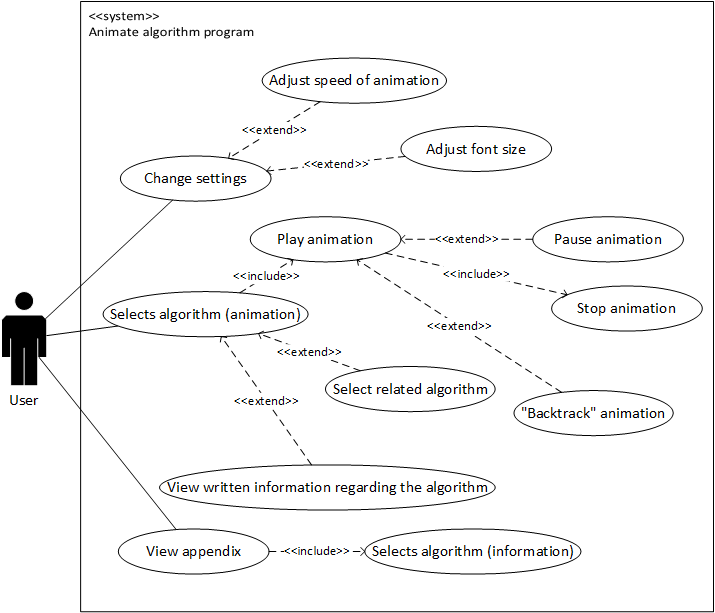
\includegraphics[scale=1]{images/report_images/useCaseDiagram.png}
\caption{The system use case diagram}
\label{useCaseDiagram}
\end{figure}

According to the use case diagram on figure \ref{useCaseDiagram}, firstly, the user can change the settings in the program, by changing features such as the speed of the animation, or the font size displayed in the program. This allows the user to work within the environment that is most comfortable for them. 

Other than changing the settings, the user can also select an algorithm which they wish to learn. This will lead them to the page where the animation of the algorithm is. From here, the user can manipulate the animation, by pressing controls such as play, pause, stop and ``backtrack''. For more information in regards to these controls, refer to the \todo[color=orange]{add some glossary or some sort}. From this page, the user can also access the algorithms which are \textit{related} to the one in question, if they ever wish to do so. This will lead to the page of the algorithm along with its animation.

Other than the settings and the animated feature, if the user ever wishes to know more about the algorithms, the user can view them in the appendix within the program. In the appendix, the user will find all the algorithms available in the program in a list. Once the user selects a particular one they wish to see, the page will display a fuller information in regards to the algorithm. This includes the written up information, and might also involve a few images as well.

\newpage

% --------------- FLOWCHART -------------------
\section{System flowcharts}
In this section, I have included the flowcharts of the program, to display the how the program flows in general, and how decisions controls its following events. 

\subsection{Main flow of the program}
The flowchart below on figure \ref{mainFlowChart} shows the overall flow of the program itself. The three main modules which makes up the program, i.e. change settings, view the animation of algorithms, and the appendix, are grouped in its respective subprocesses. Each subprocess will be described more in detail in sections \ref{sec:flowchartAnimation}, for the animation module, and \ref{sec:flowchartAppendix} for the appendix module.

\begin{figure}[H]
\centering
\hspace*{-1cm}
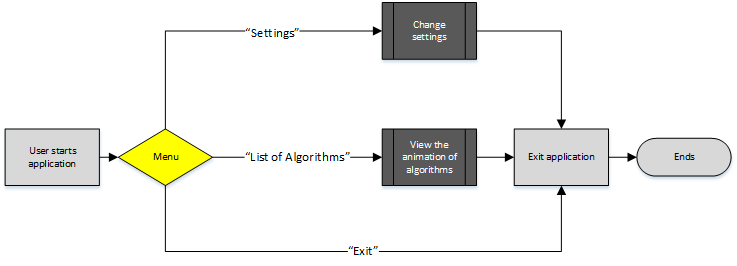
\includegraphics[scale=1]{images/report_images/flowchartMain.png}
\caption{The flowchart of the whole system.}
\label{mainFlowChart}
\end{figure}

On the main flow chart below, the user first starts the application, which then brings them to the main menu. From here, the user can select up to three features they wish to use, which are \textit{Settings}, \textit{List of Algorithms}, and \textit{Appendix}. The user can also choose to exit from the main menu, by selecting \textit{Exit} which then closes the whole application.

\subsection{Flow of the animation module} \label{sec:flowchartAnimation}
The animation module is admittedly the main feature of the program which will be heavily concentrated during the course of the implementation of the project. The user first selects the \textit{List of Algorithms} button, that leads to the animation module. From here, a list of the algorithms are classified between 3 main paradigms and a sorting algorithm into different sections for user feasibility purpose. When the user selects an algorithm they wish to learn more about, the program would lead them to a page where the animation is, and a brief description about the algorithm shown in the \textit{Information} section placed below the animation. 

The program will first prompt the user either to enter their own specific input, or the generate a random value instead. When the user decides to add their own input, there will be a specific limit assigned to the algorithm. If the input exceeds the limited amount, the program will throw an error message to inform user that the input was unacceptable, and requests the user to add an input that does not exceed the assigned limit. On the other hand, if the user selects the \textit{Generate random value} button instead, the program would then generate a random value within the limited amount assigned, and input those value into the animation.

Once an input has been either retrieved, the user then will able to play the animation by pressing the play button. Whilst the animation is at its \textit{playing state}, the user can control the animation by either \textit{pause}, \textit{backtrack}, or \textit{stop} the animation. The state of the animation depends on the type of controls that have been selected by the user. To view the description of each control available in the animation page, below on table \ref{tab:animationControls} that shows the outcome of the animation's state when a particular control button has been selected by the user.

\begin{table}[H]
\caption{The list of animation controls.}
\begin{center}
%\begin{tabular}{cc}
\begin{tabular}{| p{4cm} | p{11cm} |}
		\hline
		\textbf{Control} & \textbf{Description} \\ \hline
		Play & This button simply initiates the animation. This button is only available for use when the animation is either at its initial stage, \textit{paused}, or \textit{stopped}. \\ \hline
     Pause & When a paused button is activated whilst the animation is playing, the animation stops temporarily. The stopped time will be saved, and will continue from that time if whenever the user chooses to play the animation. User can only pause the animation when the animation is being played. \\ \hline
     Backtrack &  This is a unique feature that comes in with the program. As the animation is animated through the use of \textit{iterations}, these iteration values will be counted and stored programmatically. When a user clicks this button, the iteration counter, \textit{i}, will be brought back to the previous iteration, which is \textit{i - 1}. Once it goes back to its previous iteration, the animation will be brought to its \textit{paused} state. From here, the user can press \textit{play}, which will initiate the animation from that particular state. \\ \hline
     Stops &  A stopped button will completely halt the process of the animation. Its final playing state will be discarded once a stop button is selected. \\ \hline
\end{tabular}
\end{center}
\label{tab:animationControls}
\end{table}

\begin{landscape}
\begin{figure}[H]
\centering
\hspace*{-2cm}
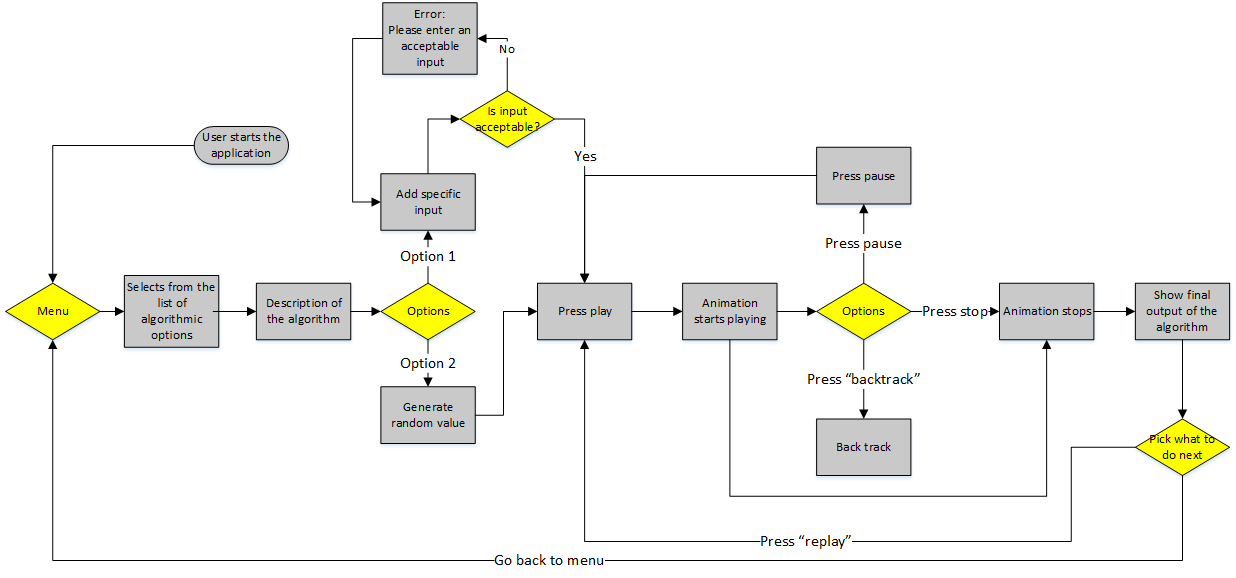
\includegraphics[scale=0.9]{images/report_images/flowchartAnimation.png}
\caption{The flowchart of the animation module.}
\label{flowchartAnimation}
\end{figure}
\end{landscape}

\newpage

\subsection{Flow of the appendix module} \label{sec:flowchartAppendix}
Finally, the last module would be the appendix module, which will contain the supplementary material in regards to the algorithms that are used in this program. This basically lists all the algorithms that are used, and users can select any algorithm within that list to view more information about the algorithm.

\begin{figure}[H]
\centering
%\hspace*{-1.5cm}
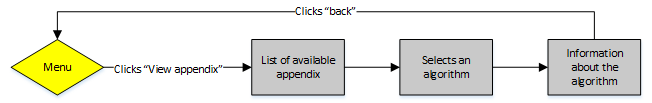
\includegraphics[scale=1]{images/report_images/flowchartAppendix.png}
\caption{The flowchart of the appendix module.}
\label{flowchartAppendix}
\end{figure}

The flowchart on figure \ref{flowchartAppendix} refers to the sequence of events that are involved within the module. First, from the main menu, as when the user selects \textit{View appendix}, the program then brings the user to the list of all the available appendix found in the program. The user then could select the algorithm they wish to find out more about, by clicking one from the list. This will then lead the user to the page that predominantly presents the detailed information in regards to the algorithm in question.

\newpage

% --------------- UI DESIGN -------------------
\newpage
\section{Graphical User Interface design of the system} \label{uiDesign}
\subsection{Program start page}

\begin{figure}[H]
\centering
%\hspace*{-1.5cm}
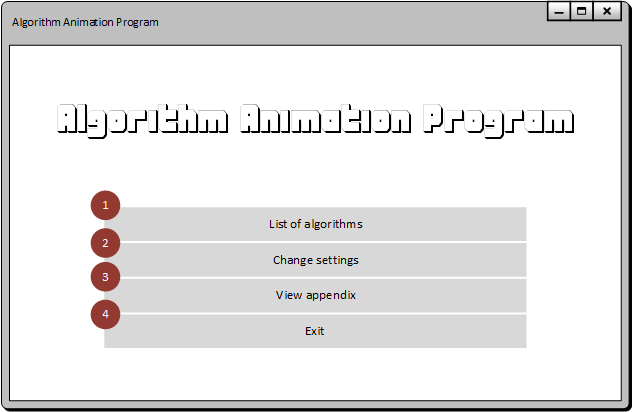
\includegraphics[scale=1]{images/report_images/uiStartWindow.png}
\caption{The start page of the program}
\label{uiStartWindow}
\end{figure}

As the program first initiates, the UI design shown in figure \ref{uiStartWindow} will be the start page of the application. The start page displays the main menu of the application. 

\begin{enumerate}
\item The \textit{List of Algorithm} button leads the user to the list of algorithms. In this list, user can select whatever algorithm they wish to learn. 
\item The \textit{Change settings} button on the other hand, leads the user to a settings page.
\item The \textit{View appendix} page brings the user to the main appendix list, which lists all the algorithms that is shown within the program.
\item Finally, the \textit{Exit} button would close the whole application, if the user selects it.
\end{enumerate}

\newpage

\subsection{Settings page}

\begin{figure}[H]
\centering
\hspace*{-0.5cm}
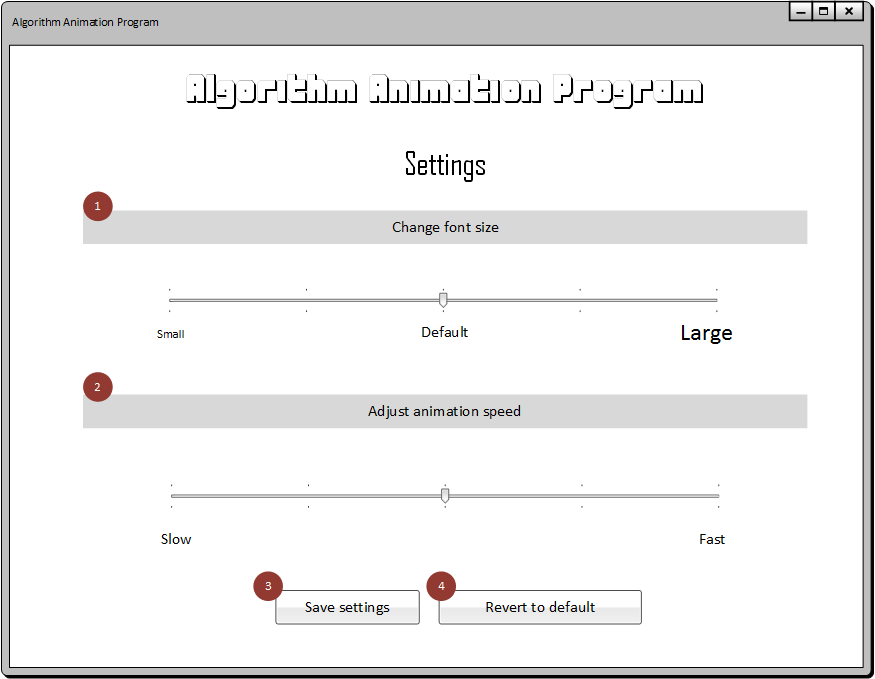
\includegraphics[scale=0.8]{images/report_images/uiSettings.png}
\caption{The settings page.}
\label{uiSettings}
\end{figure}

On the \textit{Settings} page, users can adjust several features of the program, such as the font size, and the animation speed. The reason for having a settings page is to ensure that the users are working in an environment that they are most comfortable in.

\begin{enumerate}
\item One of the features the user can change is the font size. In order to change the font size, the user is to use the slider below. From the leftmost part of the slider is the smallest size of the font, which is size 9pt. The default size on the other hand is 12pt, followed by the largest possible size is 18pt. 
\item Secondly, the user can also change the animation speed. Initially, the animation will be running on a default speed of \todo[color=orange]{find the specific speed of the animation!}. However, if the speed is either too fast or slow for the user, the user could always adjust the speed by sliding to the leftmost bit of the slider for slower speed, and rightmost for a faster speed.
\end{enumerate}

\subsection{List of algorithms page}

\begin{figure}[H]
\centering
\hspace*{-0.5cm}
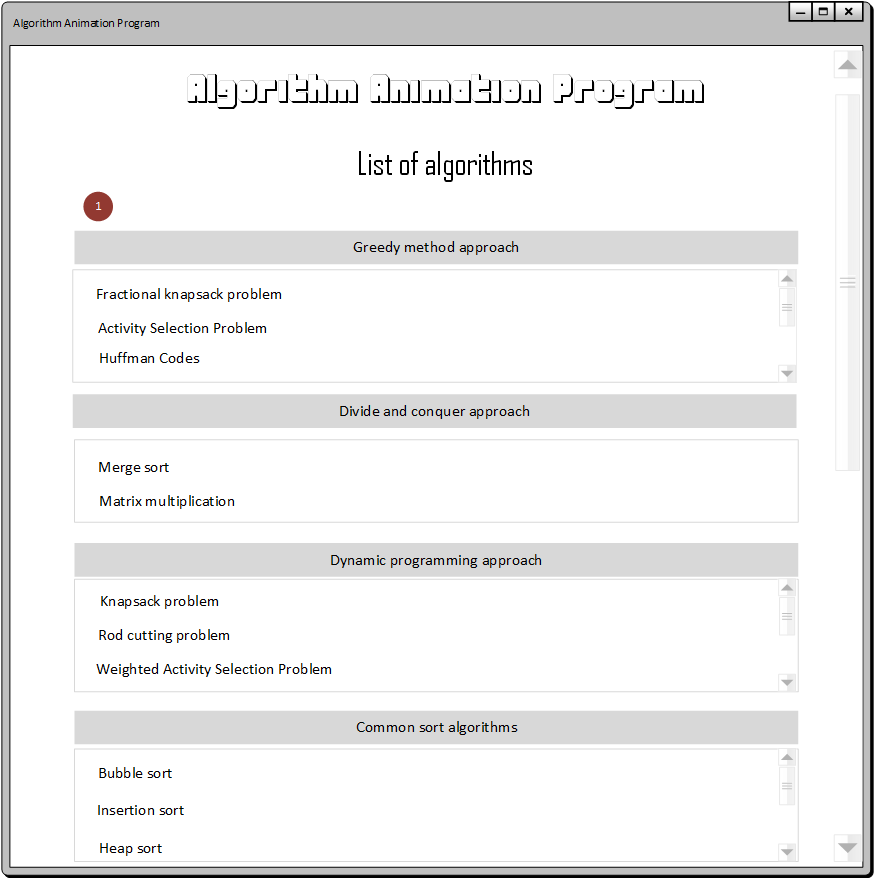
\includegraphics[scale=0.8]{images/report_images/uiListOfAlgorithms.png}
\caption{The page that shows the list of algorithms available for animation.}
\label{uiListOfAlgorithms}
\end{figure}

In this page basically shows the list of all the algorithms that are available in animation. These algorithms are also to be classified between the three main algorithmic paradigms, which are \textit{greedy method}, \textit{divide and conquer}, and \textit{dynamic programming} approaches. Also, another classification would be the sorting algorithms will be included in the list as well.

\begin{enumerate}
\item Shows the list of all the algorithms available. These algorithms are also classified according to its respective algorithmic paradigms. Users can click any of those algorithms displayed in that list if they wish to learn more about them.
\end{enumerate}

\subsection{The page of the animation of the algorithm selected}

\begin{figure}[H]
\centering
\hspace*{-0.5cm}
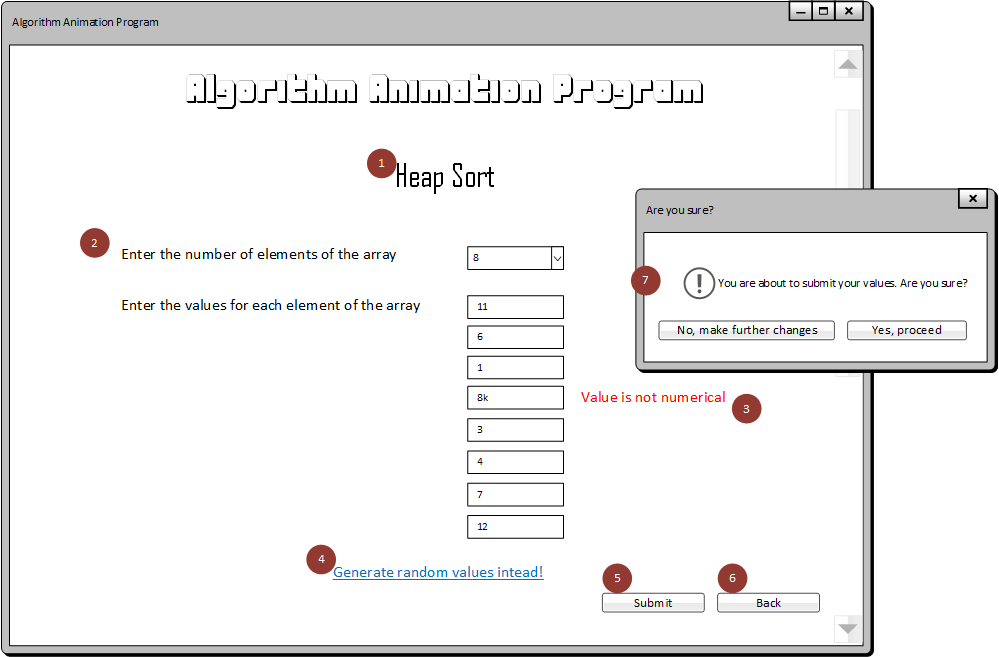
\includegraphics[scale=0.7]{images/report_images/uiInputAnimation.png}
\caption{The page that shows requests the input from the user before starting the animation of the algorithm.}
\label{uiInputAnimation}
\end{figure}

\begin{enumerate}
\item The title of the algorithm in question.
\item The form page of the list of input that is required for the heap sort animation.
\item As all fields are equipped with validation, it will throw an error message in regards to the field if it happens to receive the wrong input. For this case, the user fails to insert a numerical value.
\item Another option instead of adding the user's own input is to generate random values for the animation.
\item This button submits the values and proceeds to the next page, shown in figure \ref{uiAnimation}.
\item This button simply brings the user back to the list of algorithms.
\item This dialog will be prompted once the user clicks the \textit{Submit} button. This is to ensure that the user is happy with the input they have given. From here, if they click \textit{No, make further changes}, the dialog will close, and the page remains the same. If the user clicks \textit{Yes, proceed}, the program will proceed to the next page, which is shown in figure \ref{uiAnimation}.
\end{enumerate}

\begin{figure}[H]
\centering
\hspace*{-0.5cm}
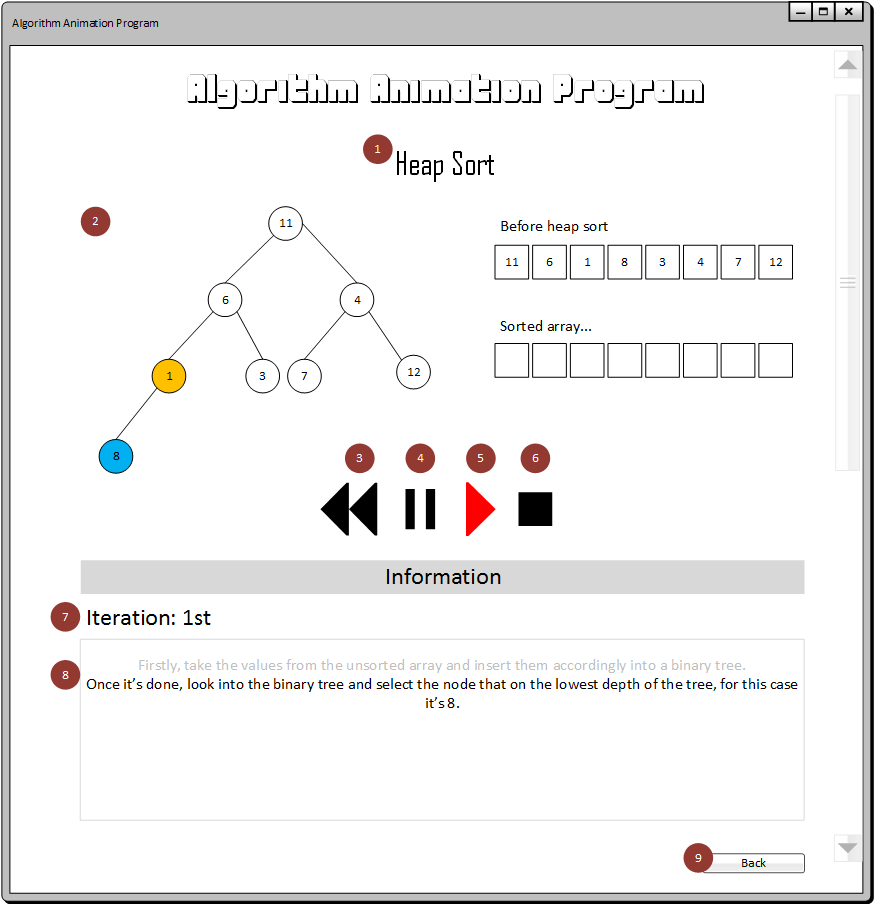
\includegraphics[scale=0.8]{images/report_images/uiAnimation.png}
\caption{The page that shows the animation of the algorithm.}
\label{uiAnimation}
\end{figure}

\begin{enumerate}
\item The title of the algorithm in question.
\item The section of the page where the animation of the algorithm is carried out.
\item The backtrack button.
\item The pause button.
\item The play button. Turns red when the animation is at the \textit{playing state}. This applies to other control buttons as well.
\item The stop button.
\item The number of iteration the animation is currently at. Every time the animation finishes its \textit{main loop}, the iteration counter is added, and it will be displayed here.
\item The area where a written information regarding the animation is displayed. Every time an animation displays something new, a new text block is displayed here, along with the numbers (variables) involved the animation. Once the animation has moved on to the next step, the text mentioned will be greyed out, as the new text will be the one that is emphasized. 
\item The button simply brings the user back to the previous page which would be the main list of algorithms. Whatever that is played in the animation will be discarded.
\end{enumerate}

\newpage

\begin{figure}[H]
\centering
\hspace*{-0.5cm}
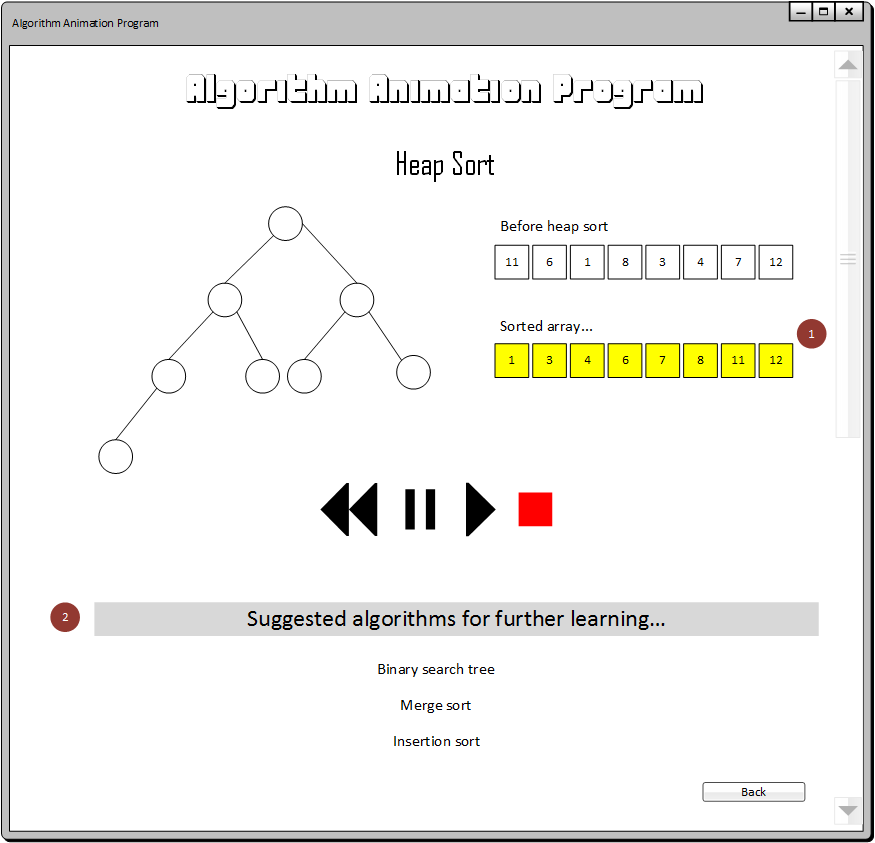
\includegraphics[scale=0.8]{images/report_images/uiAnimationDone.png}
\caption{The page's layout when the animation has finished playing.}
\label{uiAnimationDone}
\end{figure}

\begin{enumerate}
\item The animation stops right when the array has been fully sorted (only applies in sorting algorithms), or in general, has satisfied its respective goal(s). For this example, the sorted array is highlighted in yellow to show that the values in the array has been fully sorted.
\item Secondly, once the animation has ended, it also suggests the user on algorithms that are closely related to the current one for a comprehensive learning experience.
\end{enumerate}

\subsection{The appendix page}

\begin{figure}[H]
\centering
\hspace*{-0.5cm}
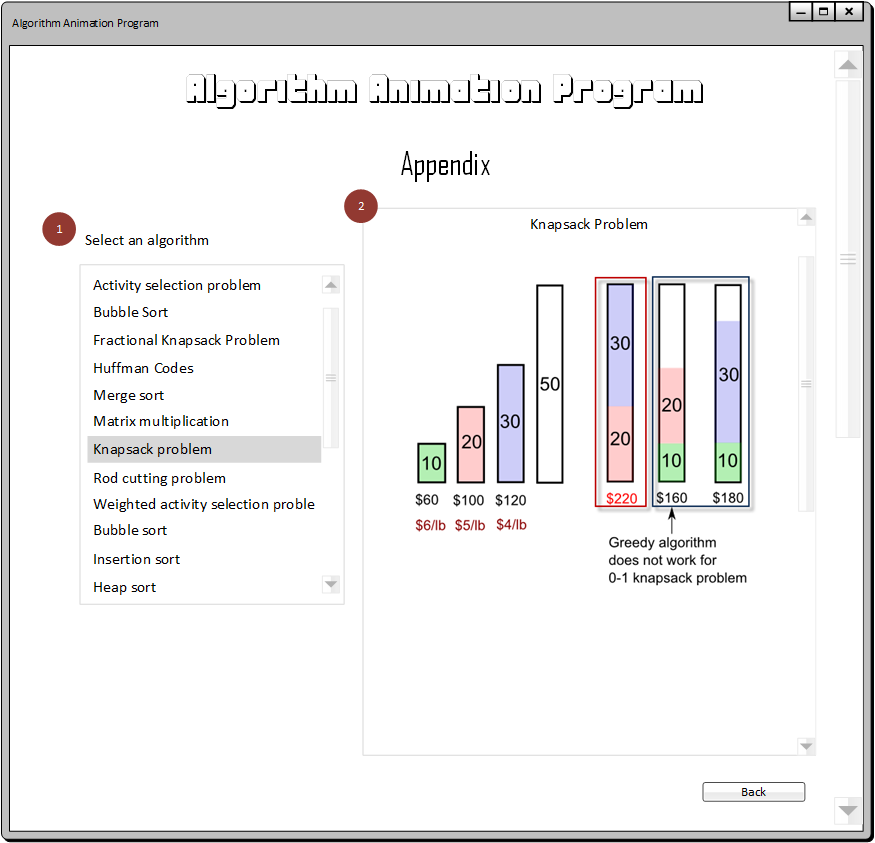
\includegraphics[scale=0.8]{images/report_images/uiAppendix.png}
\caption{The appendix page which lists the algorithms available in the program, which then shows further information regarding the algorithm.}
\label{uiAppendix}
\end{figure}

\begin{enumerate}
\item This section lists all the algorithms available in the program.
\item This section on the other hand displays whatever information about the algorithm selected from the list in no. 1.
\end{enumerate}

\newpage

% -------------- UML Class diagram --------------
\section{UML class diagram}

\newpage

%--------------- UML Sequence Diagram ----------
\section{UML Sequence Diagram}

\todo[color=yellow]{brief description about sequence diagram}


\subsection{The animation feature}
The sequence diagram shown in figure \ref{sequenceDiagramShowAlgorithmList} shows the interaction between the user and the different objects involved within the animation module found in the program. First and foremost, as the user initiates the program, the program will display the main menu by executing the \textit{displayMenu()} method. From there, the user selects (for this case) the \textit{List of algorithms} button, which leads the user to the main list of algorithms.

The user then can pick any algorithm they wish to learn from this list. For example, the uses decides to learn how the merge sort algorithm works. So the user clicks the button called \textit{Merge sort algorithm}, which then leads the user to the next page, the input request page, or known as \textit{AlgorithmAnimationInputRequest} according to the sequence diagram in figure \ref{sequenceDiagramShowAlgorithmList}.

Once the values have been inserted, the program proceeds to the animation page by calling out the \textit{displayAnimation()} method, along with the \textit{play()} method that plays the animation. Once the animation is playing, the user can manipulate the animation by using the control buttons such as the \textit{play}, \textit{pause}, \textit{stop}, and \textit{backtrack} button. Each of these controls has its own call of method, and will be called accordingly depending on which control button is pressed. 

If any control button is pressed, the program then calls out the \textit{displayAnimationRealTime()} method. This method predominantly used to run the animations, such as keeping track of the iteration(s) of where the animation is currently at, and also tracks where the timing of the animation is currently at when a control button is clicked. Of course, the latter does not apply to the \textit{stop} button, as the animation will be told to immediately reach to the end once the animation has stopped. 

Once the animation has stopped, either by the user or the animation simply reaches to its own end, the program will then give the user an option of viewing other algorithms that are similar to the one in question, by calling the \textit{getSuggestedAlgorithms()} method. The user can either click one of the suggested algorithms, or choose to go back, which brings them to the main algorithm list.

\begin{landscape}
\begin{figure}[H]
\centering
%\hspace*{-1.5cm}
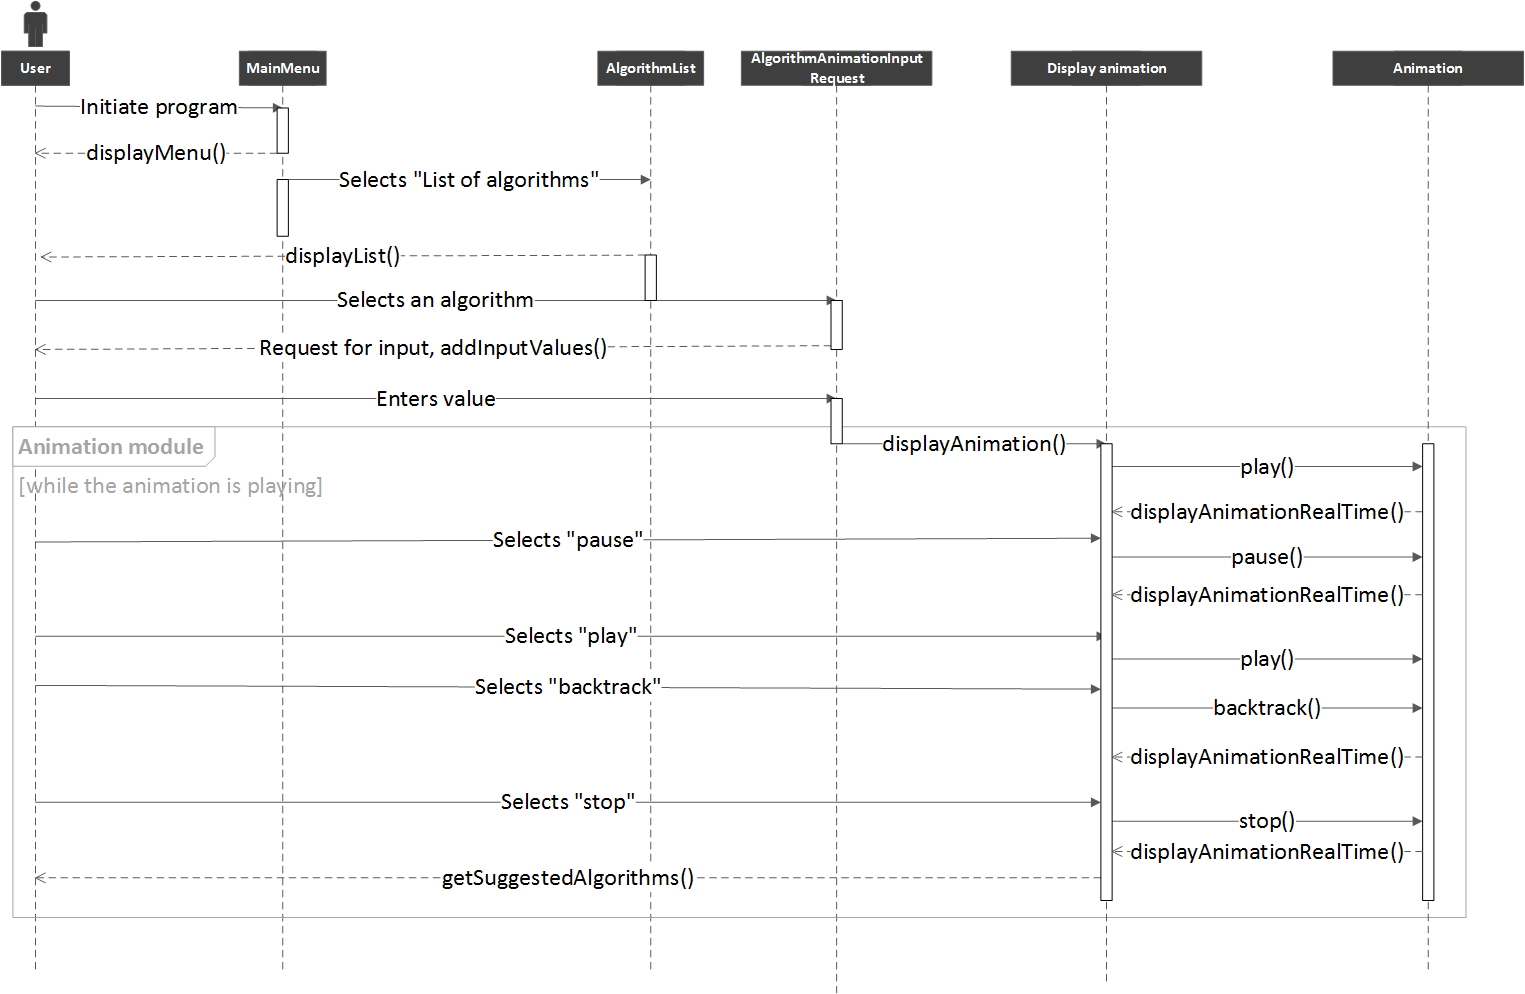
\includegraphics[scale=0.55]{images/report_images/sequenceDiagramShowAlgorithmList.png}
\caption{The sequence diagram of when the user uses the animation feature.}
\label{sequenceDiagramShowAlgorithmList}
\end{figure}
\end{landscape}

\newpage

\subsection{The settings feature}

\begin{figure}[H]
\centering
\hspace*{-1cm}
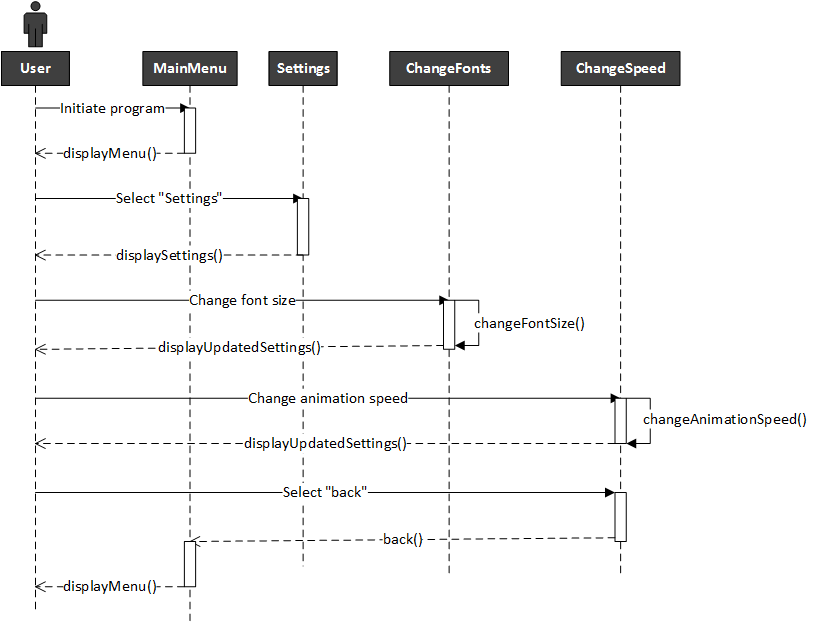
\includegraphics[scale=0.9]{images/report_images/sequenceDiagramSettings.png}
\caption{The sequence diagram of when the user uses the settings feature.}
\label{sequenceDiagramSettings}
\end{figure}

Another feature that is available in the program would be the settings feature. Based on the sequence diagram in figure \ref{sequenceDiagramSettings}, as when the user opens the program, the program will call the \textit{displayMenu()} method to display the main menu onto the client. The user then selects \textit{Settings} button, which leads them to the settings page, which would be called out by the \textit{displaySettings()} method.

Once the user is in the settings page, the user can change features such as the font size and the animation speed. If the user decides to change the font size, the \textit{changeFontSize()} method is being called out. When the method is called, it passes the parameter of the font size chosen by the user, and uses it to make necessary changes to the font size. Once that is done, the program then calls out the \textit{displayUpdatedSettings()} to change the outlook of the program to whatever that is changed. The same applies to when the speed of animation is changed, however this time, the \textit{changeAnimationSpeed()} method is called out instead. 

Once the user is done with changing the settings, they could then press the \textit{Back} button, which leads them back to the main menu. To see the graphical interface design of the settings page, do refer to figure \ref{uiSettings}, on page \pageref{uiSettings}.

\newpage

\subsection{The appendix feature}

\begin{figure}[H]
\centering
%\hspace*{-0.5cm}
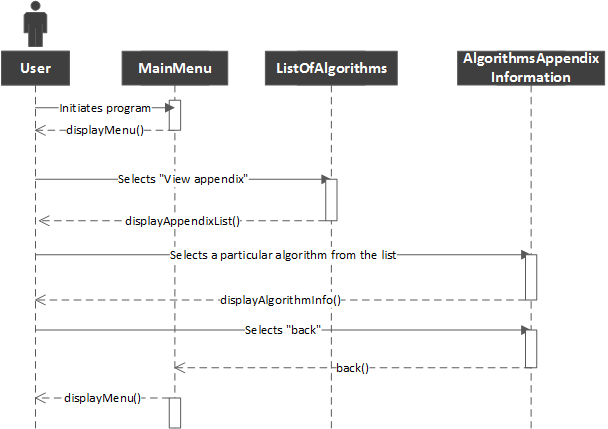
\includegraphics[scale=1]{images/report_images/sequenceDiagramAppendix.png}
\caption{The sequence diagram of when the user uses the appendix feature.}
\label{sequenceDiagramAppendix}
\end{figure}

Last but not least, the appendix would be the other feature that would be available in the \textit{Algorithm Animation} program. From the main menu, the user clicks the \textit{View appendix} button, which calls out the \textit{displayAppendixList()} method, and leads the user to the appendix page. Once the appendix page is displayed, the user could select the algorithm they wish to find out more about, within the list presented on the page. Once the user selects one, the program calls out the \textit{displayAlgorithmInfo()} with the name of the algorithm as the passing parameter, which displays the information available for the algorithm.

When the user is done, the \textit{Back} button can be selected, which leads them back to the main menu. Like before, if you wish to refer to the graphical user interface design of the appendix page, refer to figure \ref{uiAppendix} in page \pageref{uiAppendix}.

\newpage

% ------------- Algorithm animation design ----------------
\section{Algorithm animation designs}
In this section, I will present you the designs of the animations that will be included in the \textit{Algorithm Animation} program. This section is to propose an idea how the animation will look and act like, and to give a guidance on how to develop them during the implementation stage. Alongside with the design of the animation, I will also include a brief description about the algorithm, and whatever is happening within the animation.

Note that I have not included the control buttons in these designs. This section is mainly to emphasize the design of the animation of the algorithm in question. If you would like to refer to the design of the actual graphical interface within the animation page, do have a look at section \ref{uiDesign}, on page \pageref{uiDesign} for more details.

\subsection{Fractional Knapsack Problem}
\begin{figure}[H]
\centering
%\hspace*{-0.5cm}
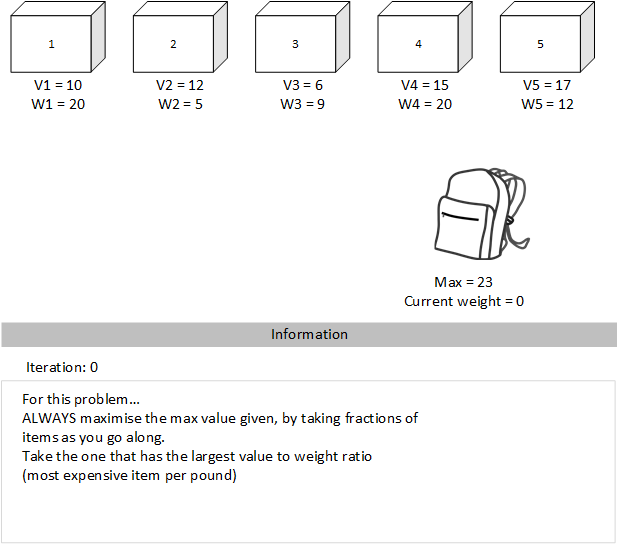
\includegraphics[scale=1]{images/report_images/animationDesignFractionalKnapsackProblem.png}
\caption{The animation design of the FractionalKnapsackProblem. This shows the initial state of the animation.}
\label{animationDesignFractionalKnapsackProblem}
\end{figure}

The Fractional Knapsack Problem is one of the algorithms that uses a combinatorial optimisation strategy in which the goal is to fill the knapsack, with fractional amounts of items until it reaches to its maximised value. This algorithm predominantly uses the greedy method approach in order to reach to its optimal solution. Within this section, I have included the design of how the animation for this algorithm will turn out to be, along with its descriptions that describes each of the different processes that happens during the play time of the animation.

The graphical interface of the Fractional Knapsack Problem algorithm shown in figure \ref{animationDesignFractionalKnapsackProblem} is the initial state of the animation. The animation consists of the items, which are represented in cubes, along with its values, i.e. weight and value of the item. Other than the items, there will also be an image of a rucksack that represents the knapsack. The knapsack has its max weight, which is the maximum amount of weight it can possible carry, and the current weight it is carrying now.

The next step of this animation shown in figure, is simply to follow the process of the animation. In this design, the animation is currently at the stage where it needs to calculate each of the items' value to weight ratio. The animation simply adds another value to each of those items called \textit{Ratio}, that shows the results to the calculation. Next would be the part of the animation is when the items are re-arranged according to their value to weight ratios.

Once the items are finally arranged, it is now time to add the items into the knapsack. The animation will represented that by dragging the item in its current iteration next to the knapsack. An arrow will then appear next to the item to represent the act of adding the item into the knapsack. When the item in question is added into the knapsack, there will be a change on the \textit{Current weight} value. 

There is an exception to this animation, that the knapsack, can no longer contain the total weight of the item in question. So, the animation program will inform the user, under the information section, that it can't insert the whole of item in question. This proceeds the animation to add fractions of the item instead, and doing a simple calculation (ratio * amount of weight left in the bag) along it as well. You can clearly see this calculation clearly above the arrow.

As when the calculation is complete, and the knapsack's current weight has reached to its max weight, the animation then comes into a conclusion. The conclusion of this algorithm is that the knapsack is finally full, and the total value that the knapsack has achieved is displayed as well. Afterwards, the animation stops here. 

\newpage

\subsection{Knapsack Problem}

\todo[color=yellow]{Brief description of the knapsack problem}

\begin{figure}[H]
\centering
%\hspace*{-0.5cm}
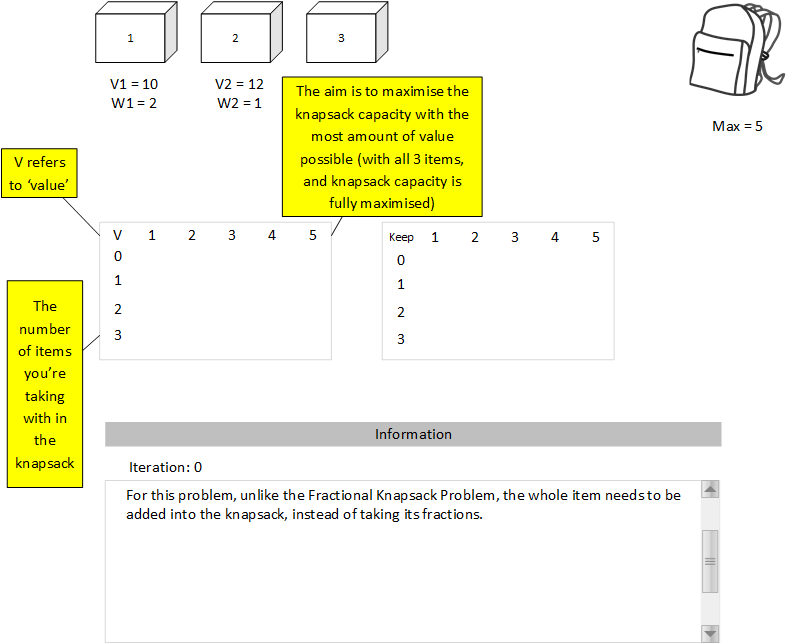
\includegraphics[scale=0.7]{images/report_images/animationDesignKnapsackProblem.png}
\caption{The initial state of the animation design of the Knapsack Problem. It shows that it is describing what the tables are.}
\label{animationDesignKnapsackProblem}
\end{figure}


As when the animation of the knapsack problem starts (refer to figure \ref{animationDesignKnapsackProblem}), few description which describes about the tables will be displayed during the animation's initial play time. Those descriptions in the yellow coloured callouts are placed around the table to describe its purpose, in order for the user to understand what they are before the actual algorithm starts. These texts will remain here for about a 30 seconds, before proceeding to the next state.

Included in this animation, other than the ones mentioned before, are the cube figures which represent the items. Along with them are its attributes, which are their respective value they are worth, and their weight. Next to it is an image of the knapsack. Show below it is its maximum capacity, and the current weight it is holding. For its initial state, the current value is always 0.

Within the \textit{Information} section, there will also be a brief description of what the algorithm is, and how is it different from the Fractional Knapsack algorithm. 

After the explanation phase has completed, the algorithm of the knapsack problem begins. The algorithm begins by applying the sum of values obtained on the first row of the \textit{value table}. Since on the left side of the table is 0, meaning that there are no items selected, all the values are returned as 0 for the first row. The texts that are inserted into the table are turned red, simply to let the users know where to look in the animation. The values are added into the \textit{keep table} as well after adding those values into the \textit{values table} previously.

As the animation proceeds to the second row, where the animation loops by doing the same thing previously on the first row. It refers to the top column, which is the weight of the knapsack to carry, which is highlighted with a green circle. Followed by the spot where the animation needs to compute the value for, which is highlighted with a red circle. 

Once filling up the \textit{value} and \textit{keep} table is completed, the algorithm looks through the keep table from the most bottom right hand side, to find out which item to keep. If the value is 1, it means that the item along that row is kept, and the total weight of the knapsack will be subtracted from the item. Do this along the column which is the maximum possible amount of capacity of the knapsack, in this case 5, until either the knapsack is full, or can no longer take in any more items. Finally once it has done that, show the total value (most optimum value you can achieve) that is taken away from the knapsack.

\newpage

\subsection{Activity Selection Problem}
\todo[color=yellow]{Description of the Activity Selection Problem}

\begin{figure}[H]
\centering
%\hspace*{-0.5cm}
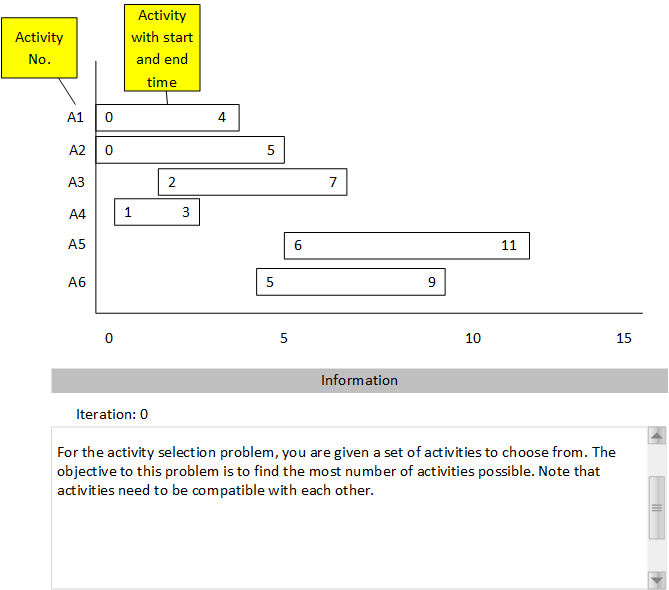
\includegraphics[scale=0.9]{images/report_images/animationDesignActivitySelectionProblem.png}
\caption{The animation design of the Activity Selection Problem.}
\label{animationDesignActivitySelectionProblem}
\end{figure}

Shown in figure \ref{animationDesignActivitySelectionProblem}, is the initial stage of the activity selection animation during its starting phase. During this phase, the animation starts off by explaining parts of the diagram, using the bright yellow callouts. Along with it, there is a further explanation about the objective of the algorithm within the information section below.

Once the explanation phase is done, the animation carries on by initiating the activity selection problem algorithm. First, it selects the activity with the earliest end time, and highlights it red. Once the activity has been chosen, it goes on by finding the other activities within the list that is incompatible with the chosen activity. These incompatible activities are then removed from the list of activities, and are greyed out in the animation to show that they are removed. Once there aren't any more activities left in the list of activities, the optimal solution to the problem has been finalised. This is when the animation ends. 

\newpage

\subsection{Merge sort}

\begin{figure}[H]
\centering
%\hspace*{-0.5cm}
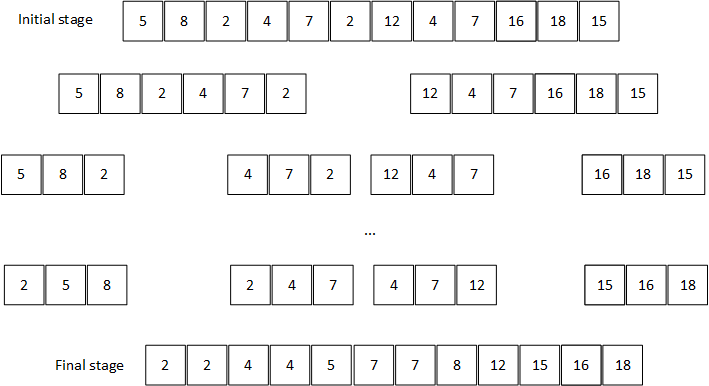
\includegraphics[scale=0.9]{images/report_images/animationDesignMergeSort.png}
\caption{Merge sort animation design.}
\label{animationDesignMergeSort}
\end{figure}

The merge sort algorithm is basically one of the sorting algorithms that uses the divide and conquer method to sort the contents of the array of values. The animation for the merge sort algorithm will emphasize mainly on the idea of a divide and conquer, which is one of the three algorithmic paradigms. 

On the input page for the merge sort algorithm, will be the number of elements in array, followed by the values for each element of the array. The animation for this algorithm will be made simple, as you can see in figure \ref{animationDesignMergeSort}. First, is to have squares that represents each element of the array. These squares will initially be set next to the other squares with values clearly shown on them.

As when the animation starts, the animation will clearly show the division it makes to divide the array into 2 parts, each side with an equal amount of elements to the other side (unless if the total number of elements is an odd number, then one side will have one more element than the other). The animation will keep on doing this until each of the elements divided will be left to one each. After which, the animation will proceed in taking the first element from the unsorted list, sorts and drags it down to another tier, and do the same for the rest until all the elements are sorted and merged as a whole. The animation then concludes by showing that it is finally sorted, and ends here.

\newpage

\subsection{Matrix multiplication}

\begin{figure}[H]
\centering
%\hspace*{-0.5cm}
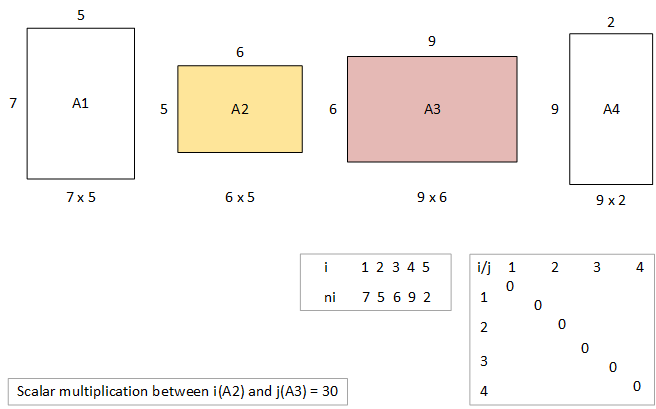
\includegraphics[scale=0.9]{images/report_images/animationDesignMatrixMultiplication.png}
\caption{Merge sort animation design.}
\label{animationDesignMergeSort}
\end{figure}

The matrix multiplication problem is classified under the \textit{optimisation problem}, that will be available in animation. This problem simply shows the algorithm on finding the most efficient way to multiply two or more matrices together, and using dynamic programming in order to find the solution. 

The input page for the animation will consist of the number of matrices to compute and the size of each of those matrices. There will be some constraint when it comes to selecting the size of the matrix however, is that, the next matrix will need to have one of its sides to be the same value as one of the sides the first matrix as well, which is a basic rule for two matrices to be multiplied with one another.

On the animation itself, it will present each matrix in a rectangular shaped figures, depending on the size that was given during the input stage. On top of each matrix will also be an identifier, which format is \textit{Mi}, \textit{i} being the number of the matrix in the list. Below each of the rectangles will show the size of the matrix, which format goes as \textit{widthSize * lengthSize}, in order to depict the size of each rectangles.

During a part of the animation, the algorithm will pick the values for \textit{i} and \textit{j}, which are the values between the 1, the first matrix, and N, where it is the number of the last matrix in the list. Between these two values, there will also be \textit{k}, which is going to be used to compute the most efficient \textit{split} to be made, in order to achieve the minimal amount of scalar multiplications between the two lists of the matrices. In every iteration of the algorithm, the animation is to use \textit{k} as a splitter, and between the two parts of the list, find the minimum amount of scalar multiplications needed. And once the minimum has been found, the algorithm will conclude its answers, and ends.

Since this problem uses dynamic programming, there is a need to add a table that goes with the animation as well. This table is what I call the \textit{i and j} table, which is a two dimensional array that makes up the size of \textit{i} and \textit{j}. This table is used to store the result of the scalar multiplications between the size of the matrices, and is used to find the most efficient solution for the problem. 

\subsection{Rod cutting problem}

\begin{figure}[H]
\centering
%\hspace*{-0.5cm}
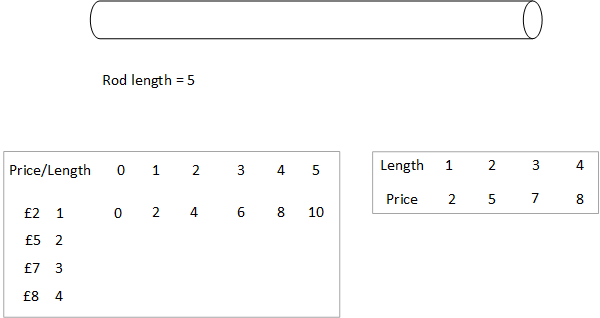
\includegraphics[scale=0.9]{images/report_images/animationDesignRodCuttingProblem.png}
\caption{Merge sort animation design.}
\label{animationDesignMergeSort}
\end{figure}

\todo[color=pink]{I left it off here}

\chapter{Review against plan}

% plan produced as part of the specification, showing what has been completed, and progress to date

% any changes to the plan should be indicated
% - not adding binary search tree
% - including human testers for the evaluation phase
% - adding the settings feature

Admittedly, there are a few changes that had deviated slightly from the specification document. One of the minor changes I have made is the exclusion of adding a binary search tree from the list of animations available the program. This is mainly to ensure that I have enough time to implement the animations for other algorithms that had been mentioned in the design chapter, under the \textit{Algorithm animation designs} section (refer to section \ref{sec:algorithmAnimationDesign} on page \pageref{sec:algorithmAnimationDesign} for the list of animation designs).

Another change that I decided to make, is to include human testers to conduct the assessment of the \textit{Algorithm Animation Program}. I believe that there is a need for me to include external parties to assess and review my product, instead of doing it myself, as specified in the specification documentation. Reason being that having someone who has a different level of knowledge and understanding in this topic to test this product, would provide me with better feedback, from their point of view, about what is good or lacking in the program. For more information about the evaluation testing, do have a look at section \ref{sec:evaluationDesign} on page \pageref{sec:evaluationDesign} for more information such as, what kinds of testers that is needed, and the sets of questions and tests that will be conducted in order to make the product ideal for use.

Finally, it is worth mentioning that I have decided to add one extra feature, the \textit{settings} feature, as I believe that this will enhance the user experience when allowing the users to work on an environment that they are most comfortable in. For now, the plans only to include in changing the font size and the speed of animation due to the time constraints that was given to me. However, I am planning to implement the settings feature that would easily allow the developers to add additional features that can be changeable, thus making the program more customisable in result, in possible further iterations of the program.

\section{Updated Gantt Chart}
In the following page shows the revised version of the Gantt Chart. It has been changed slightly to fit the plans that I have devised and documented within this design documentation. What has been predominantly change is the testing phase, which is brought much forward, and now currently aligned with the implementation stage. Of course, the testing phase is expected to require a longer time compared to the implementation, as I have set ample amount of time for the testing phase. I believe that this is one of the most important phase for me to invest on and ensure that the software will be in tip top condition before the submission.

\begin{landscape}
\begin{figure}[H]
\centering
\hspace*{-0.5cm}
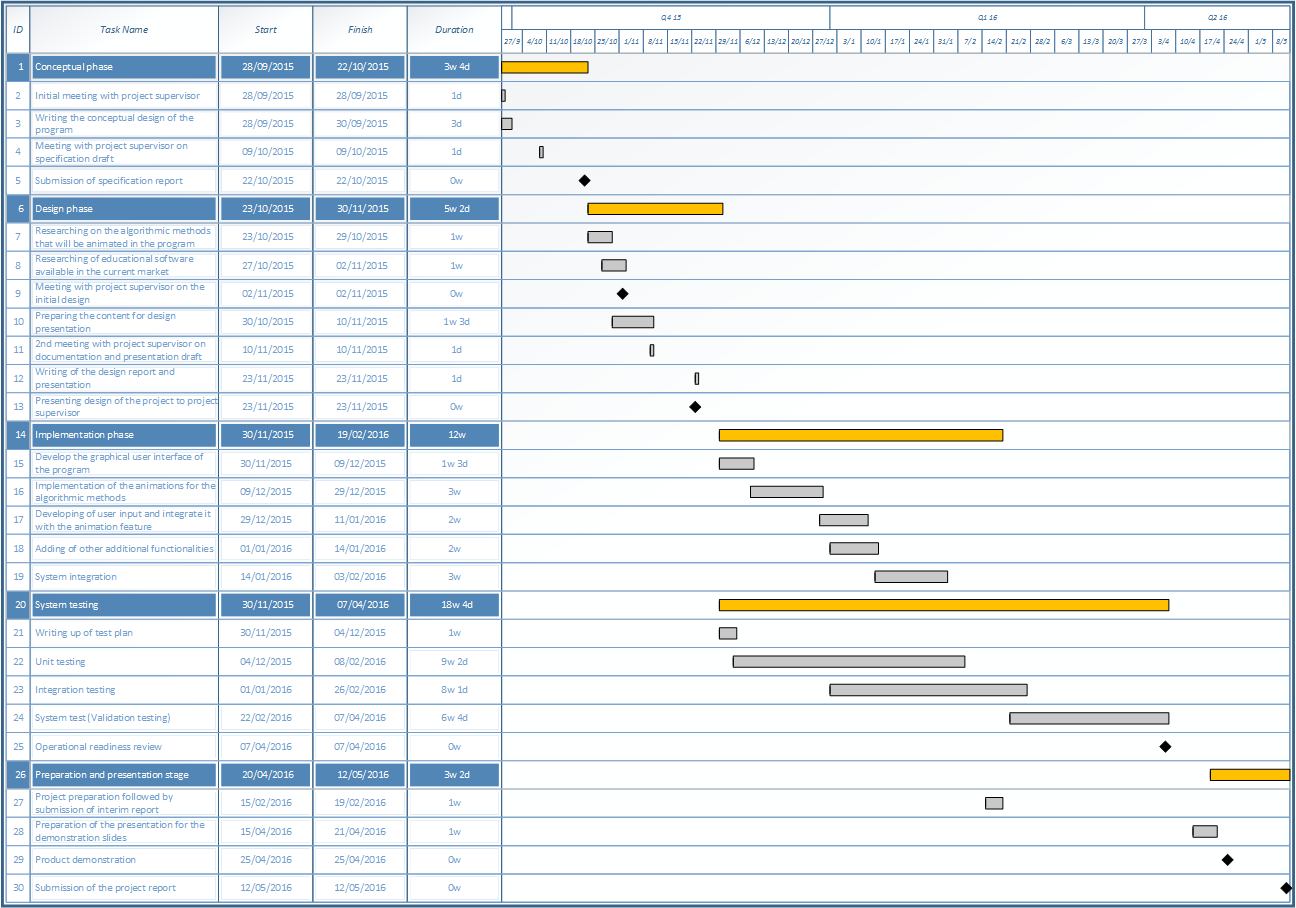
\includegraphics[scale=0.78]{images/report_images/ganttChart.png}
\caption{The updated gantt chart.}
\label{ganttChart}
\end{figure}
\end{landscape}


\todototoc
\listoftodos

\end{document}